\chapter{Appendix}


\section{Code Repository}

The code for this project can be found on UCD School of Computer Science's internal GitLab server: \url{https://csgitlab.ucd.ie/rajitbanerjee/microservice-design-patterns}

\section{Supplementary Figures}

%%%%%%%%

\begin{figure}[H]
	\centering
	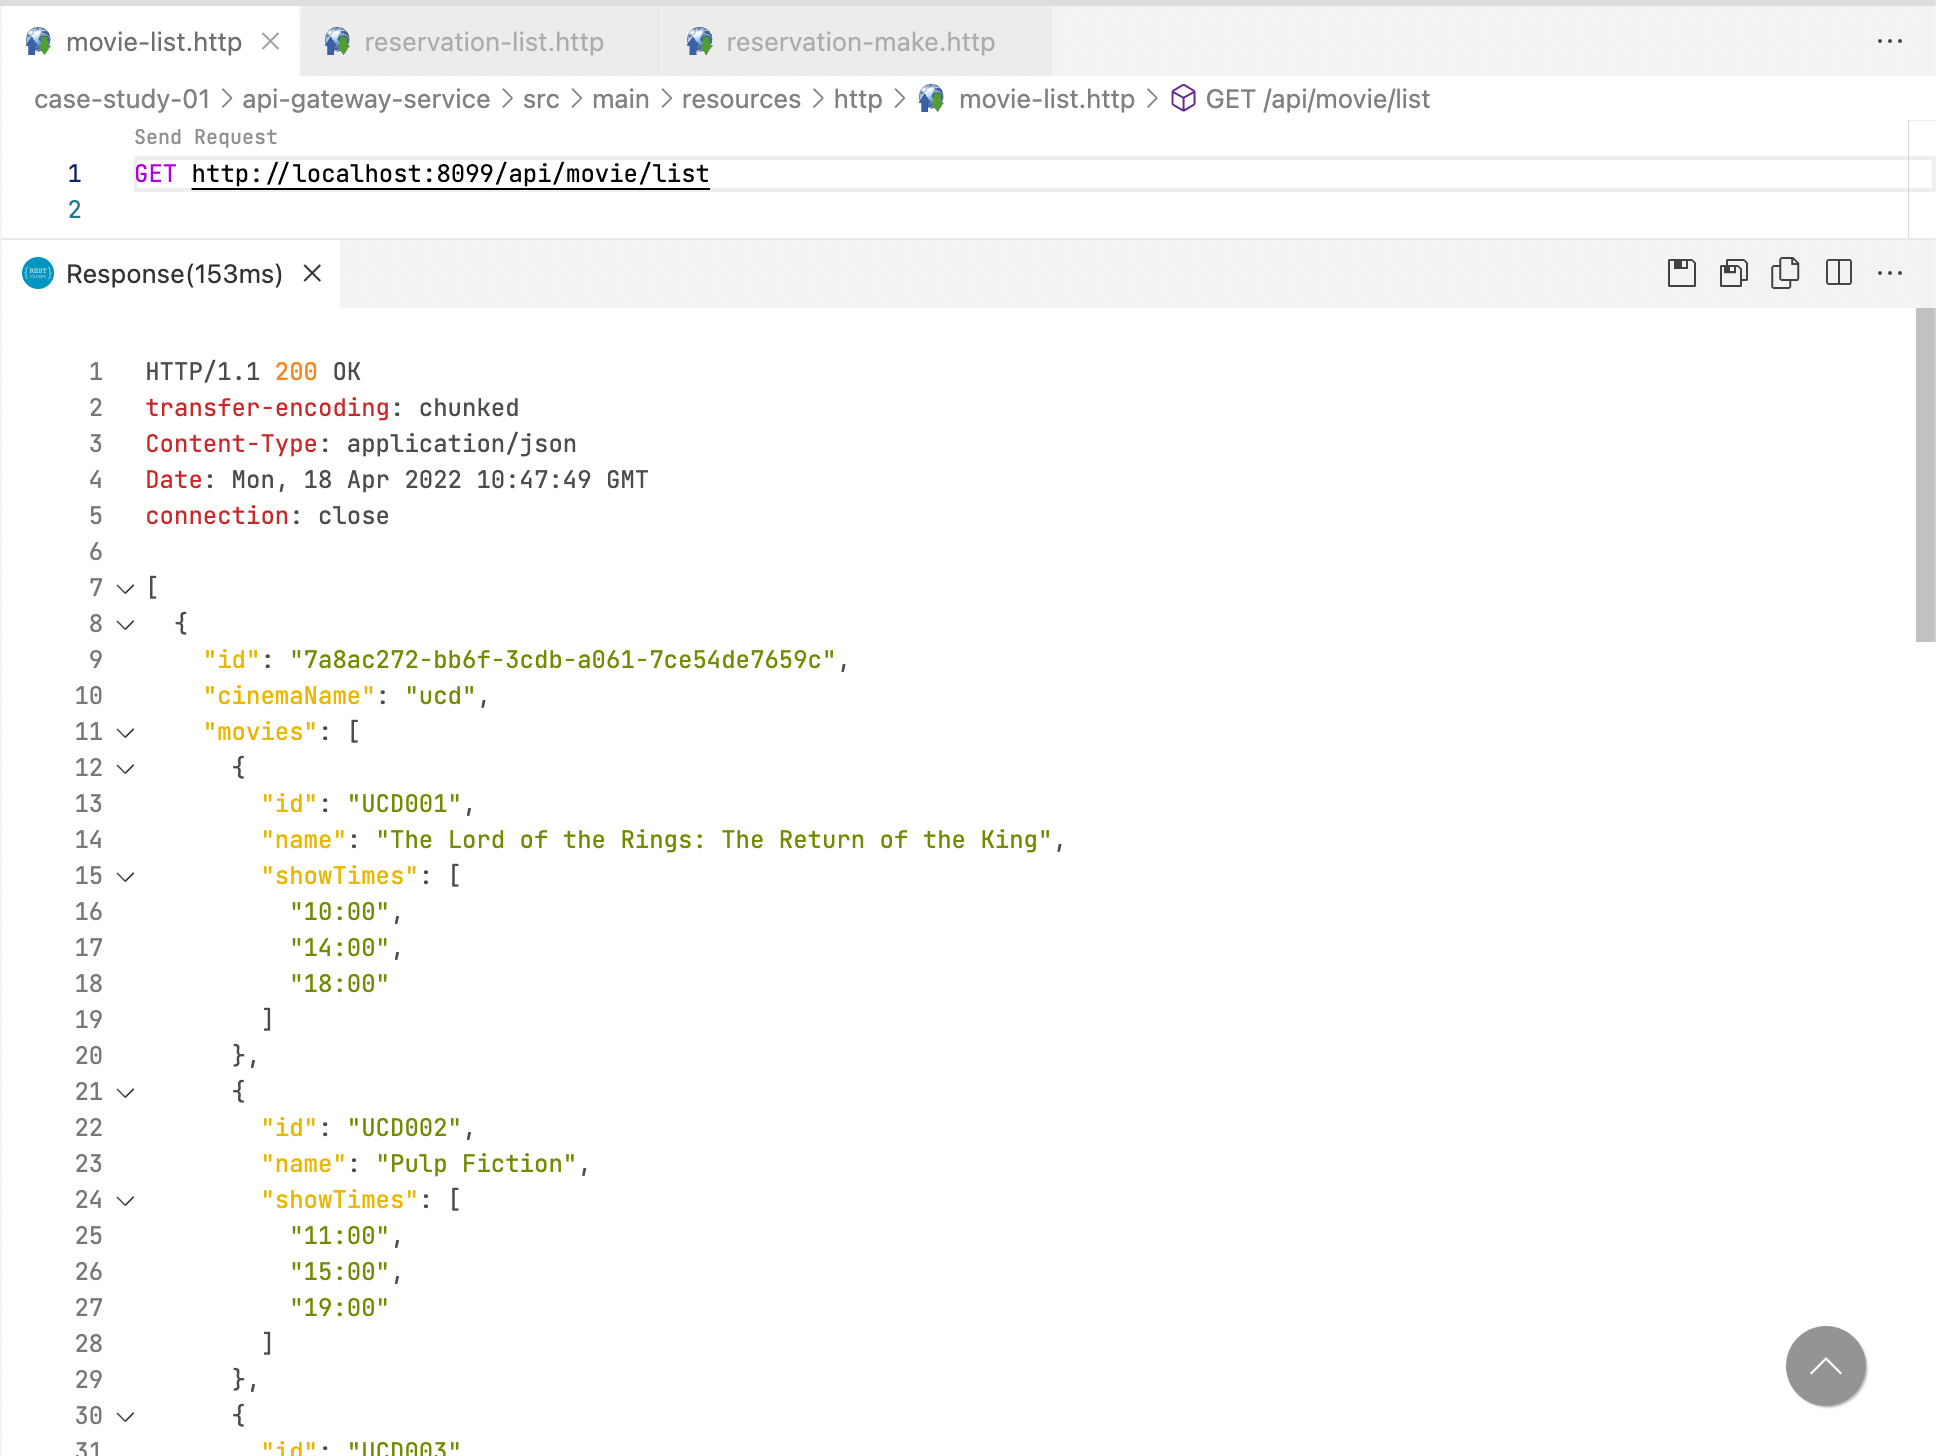
\includegraphics[width=1.0\linewidth]{./assets/images/case-studies/cs01-manual-1.png}
	\caption{Case Study 1 - manual API testing (listing all movie showtimes from various cinemas)}
	\label{fig:cs01-manual-1}
\end{figure}

\begin{figure}[H]
	\centering
	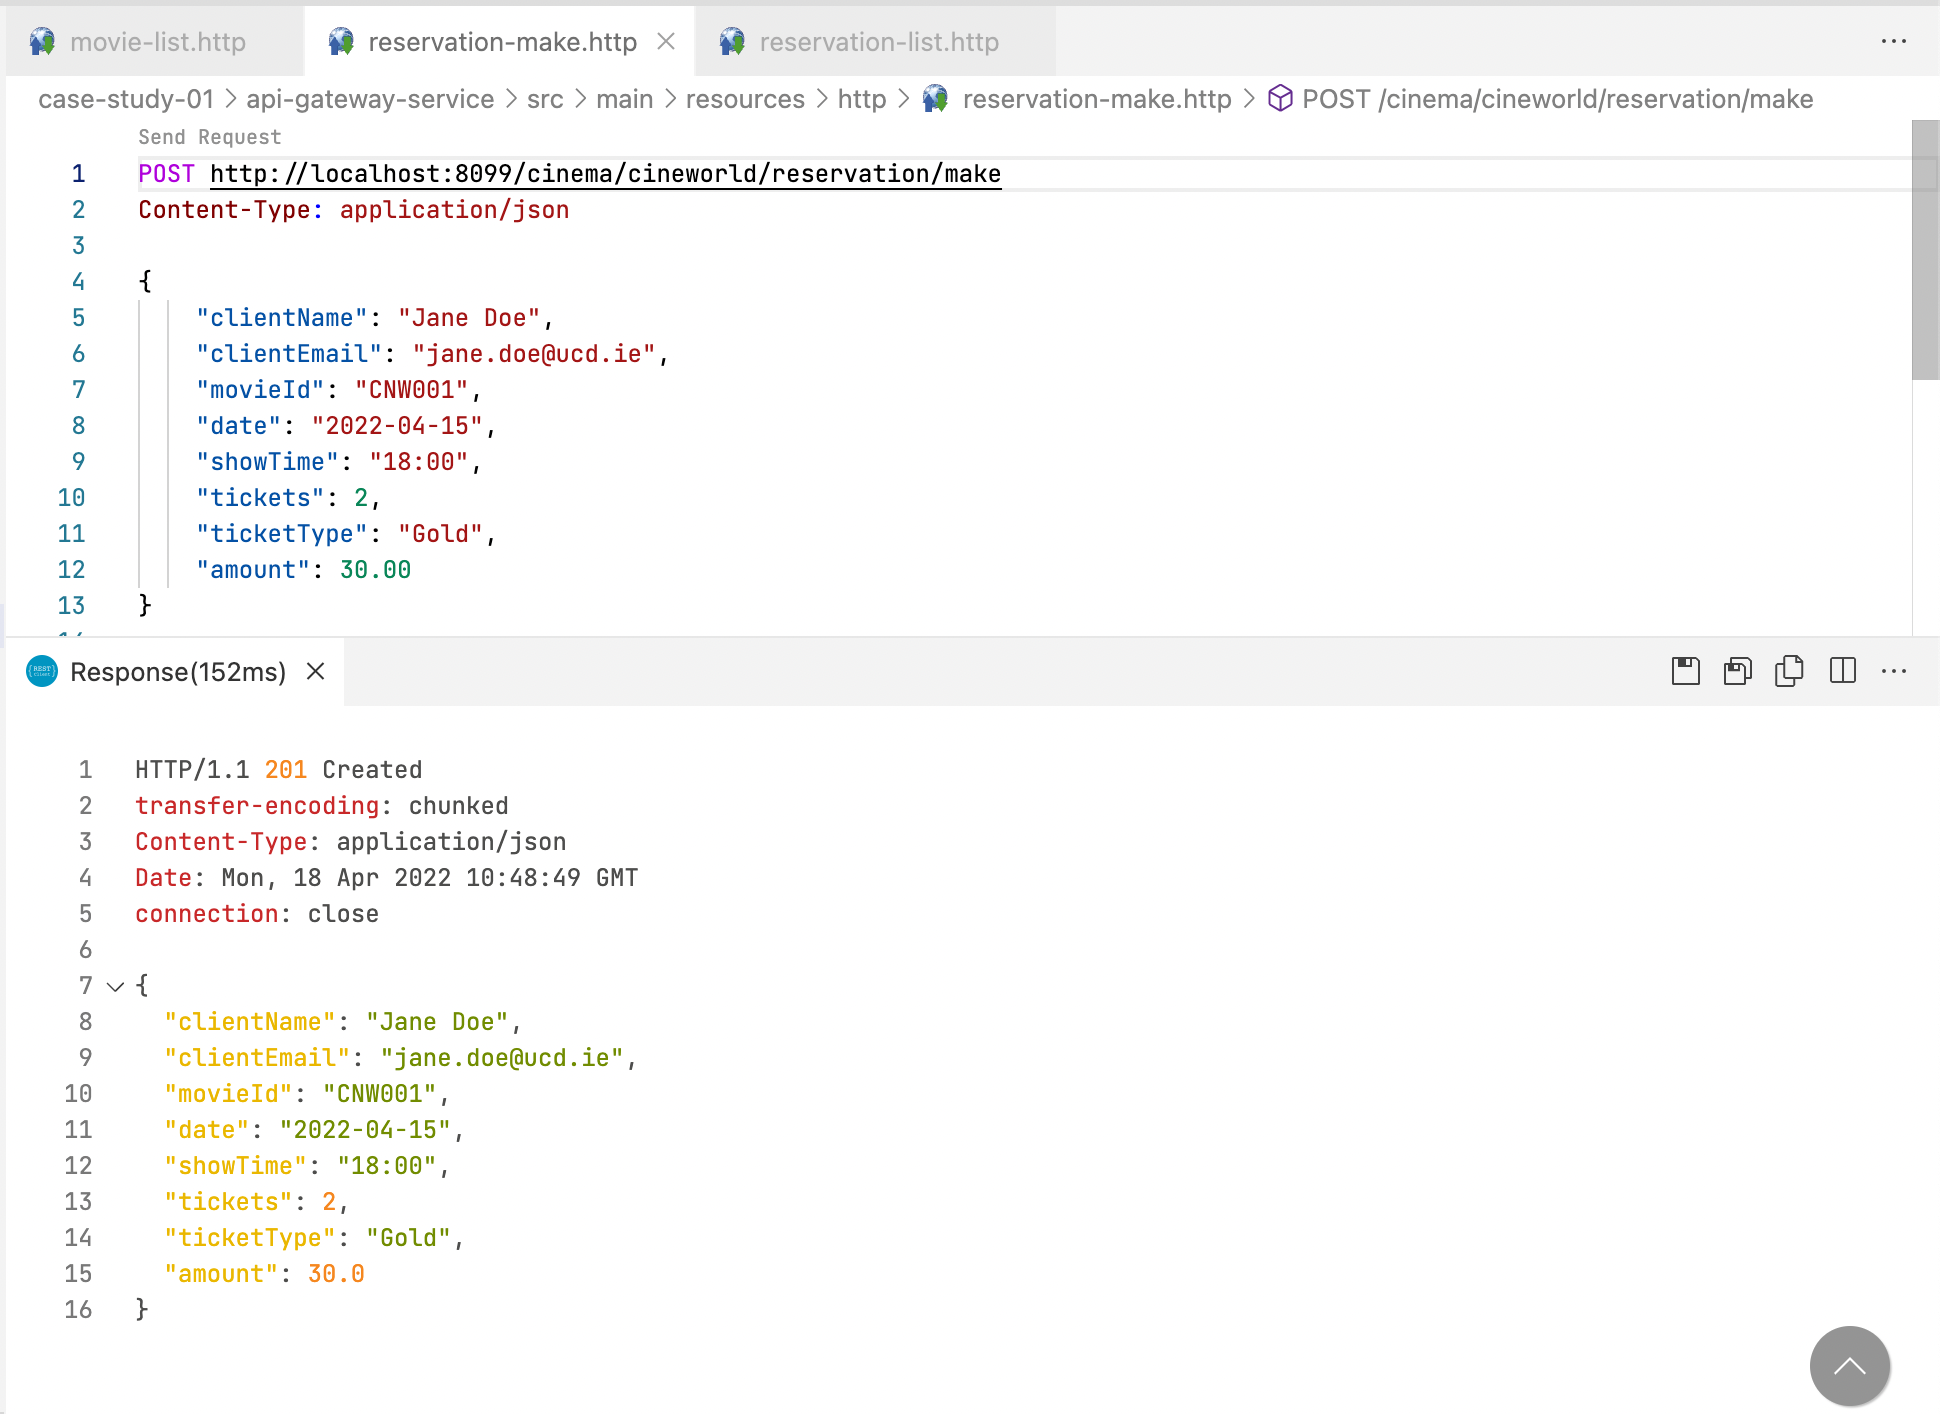
\includegraphics[width=1.0\linewidth]{./assets/images/case-studies/cs01-manual-2.png}
	\caption{Case Study 1 - manual API testing (making a reservation at Cineworld cinema)}
	\label{fig:cs01-manual-2}
\end{figure}

\begin{figure}[H]
	\centering
	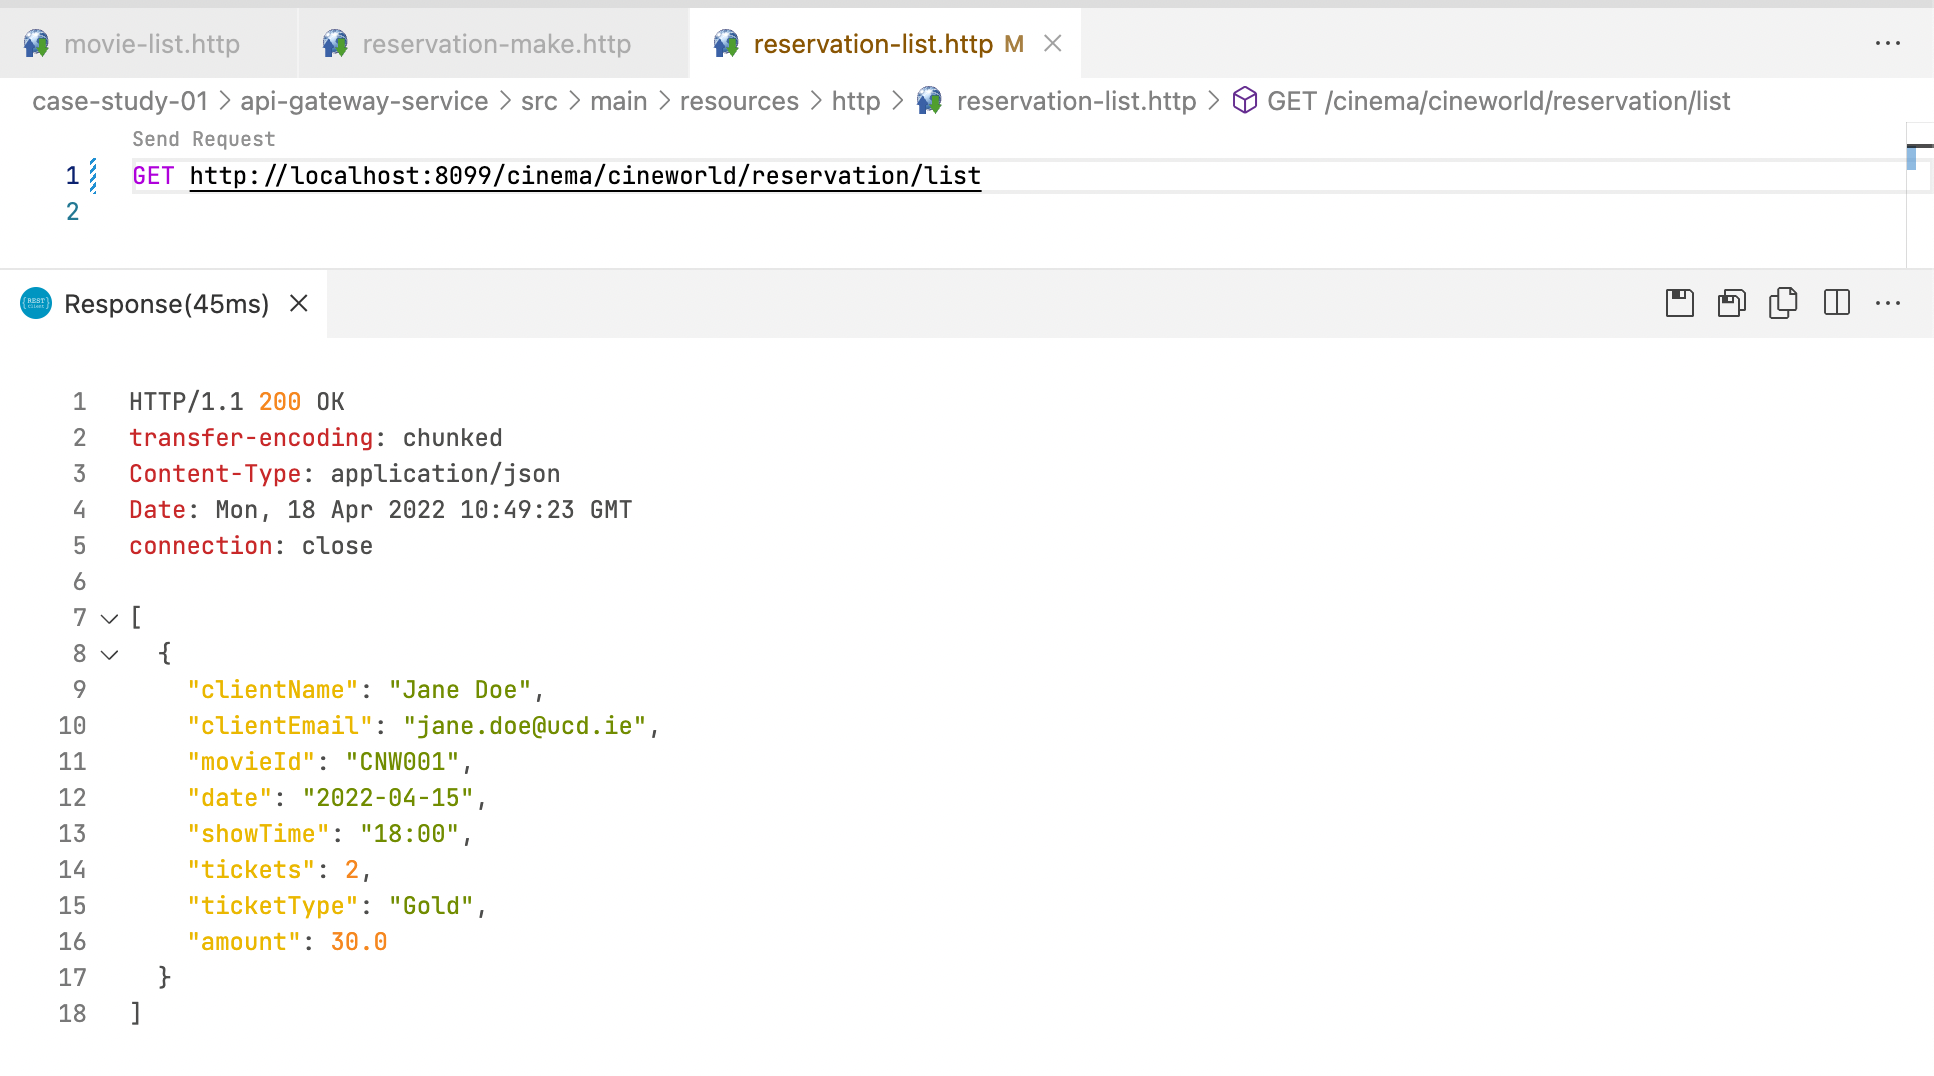
\includegraphics[width=1.0\linewidth]{./assets/images/case-studies/cs01-manual-3.png}
	\caption{Case Study 1 - manual API testing (listing all reservations at Cineworld to ensure the previous reservation was successful)}
	\label{fig:cs01-manual-3}
\end{figure}

%%%%%%%%

\begin{figure}[H]
	\centering
	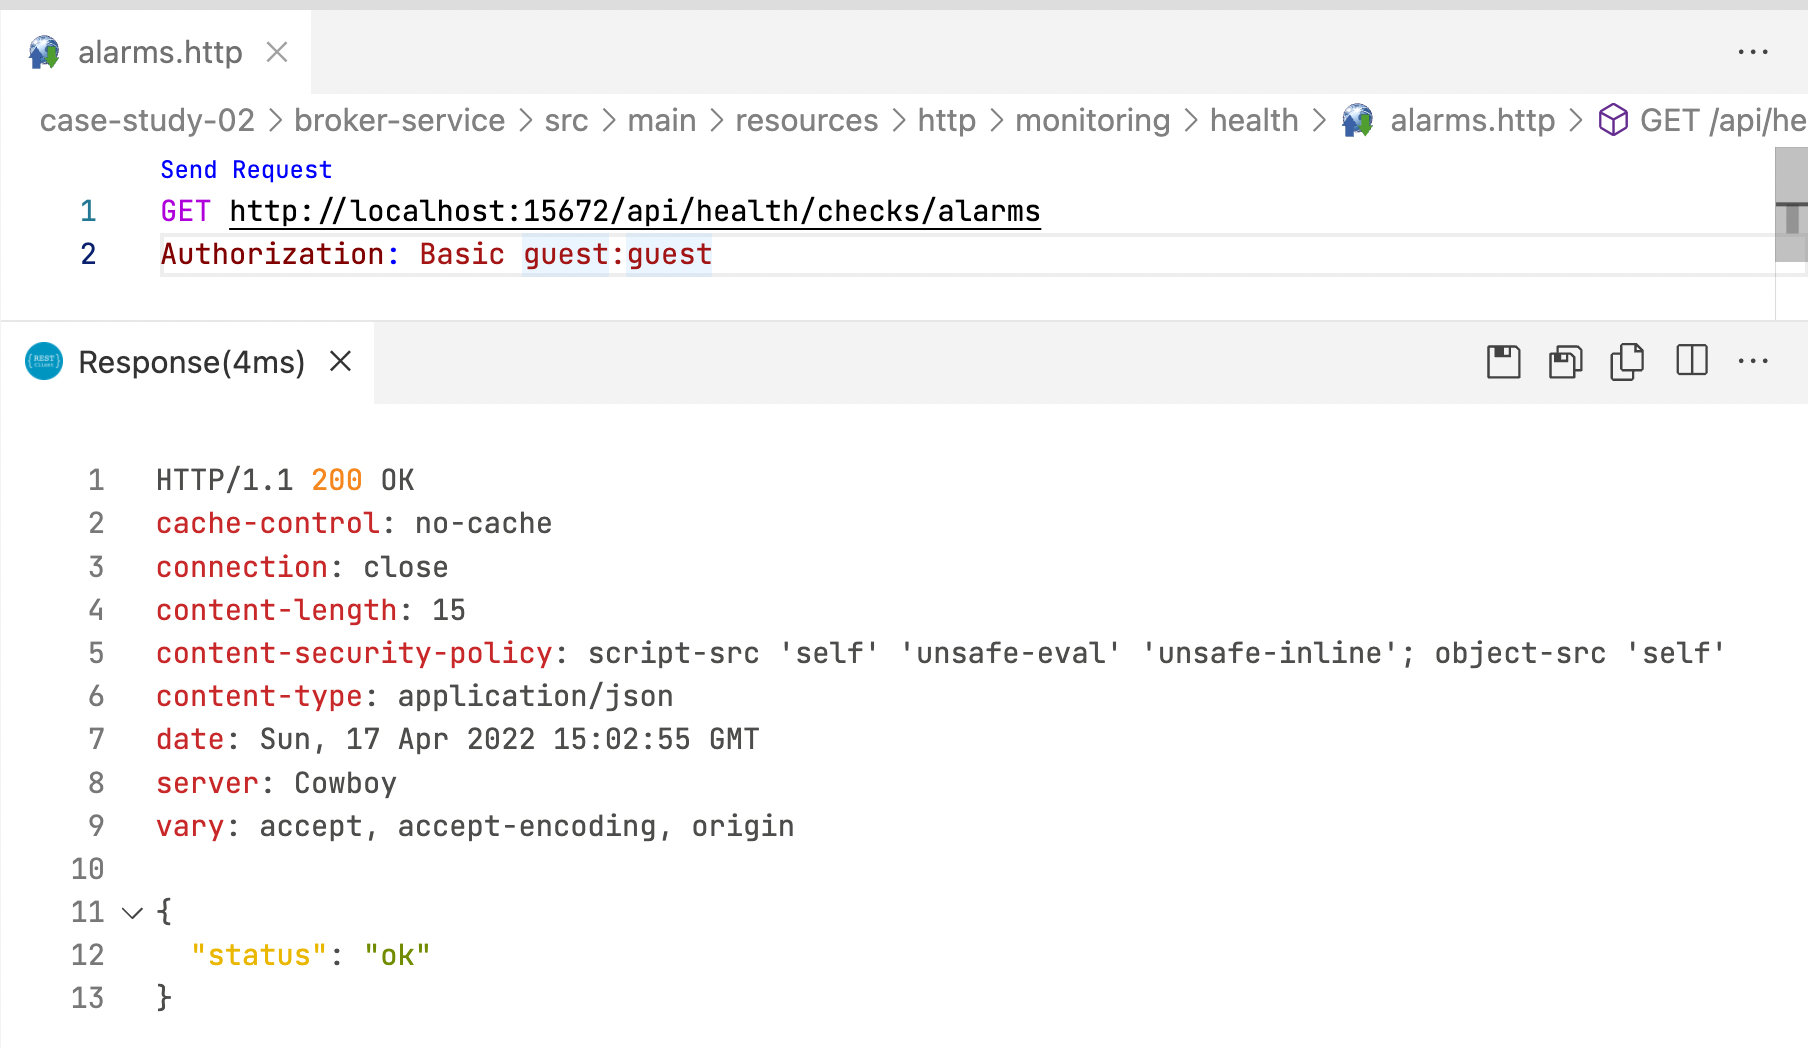
\includegraphics[width=1.0\linewidth]{./assets/images/case-studies/cs02-hc1.png}
	\caption{RabbitMQ health check - alarms}
	\label{fig:cs02-hc1}
\end{figure}

\begin{figure}[H]
	\centering
	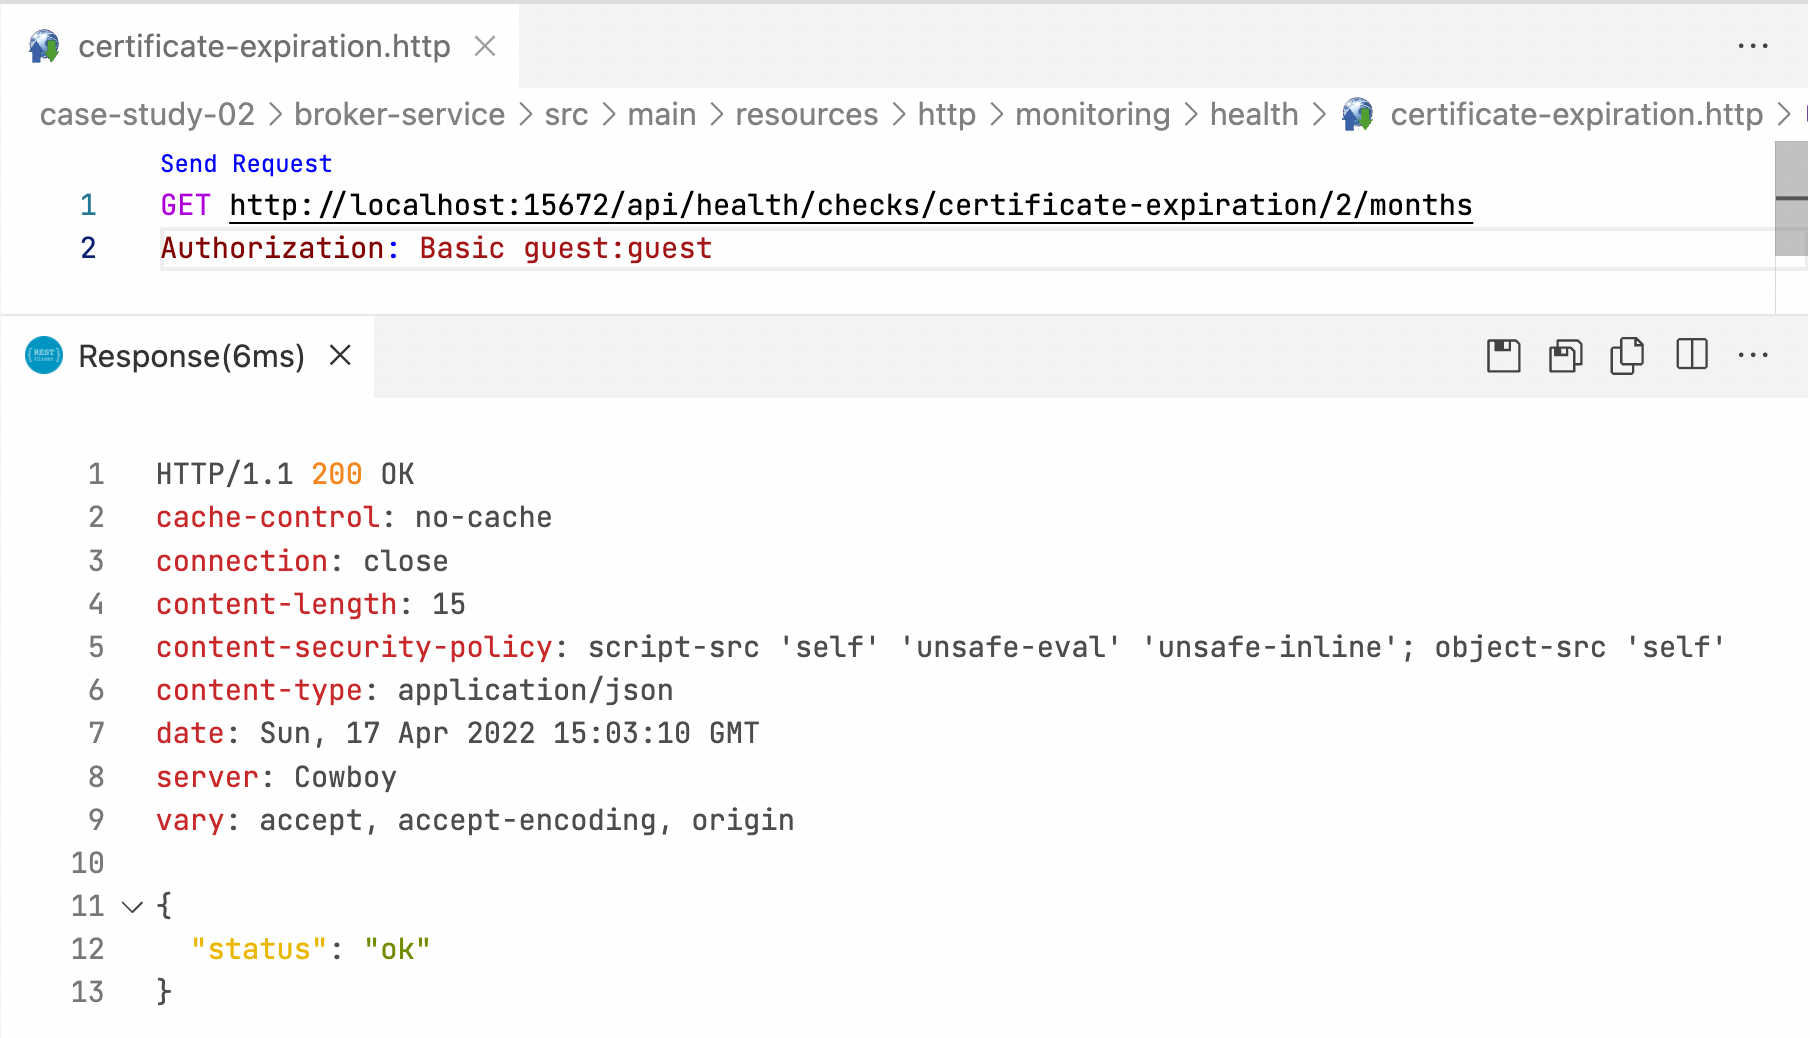
\includegraphics[width=1.0\linewidth]{./assets/images/case-studies/cs02-hc3.png}
	\caption{RabbitMQ health check - certificate expiration within a time unit (2 months)}
	\label{fig:cs02-hc3}
\end{figure}

\begin{figure}[H]
	\centering
	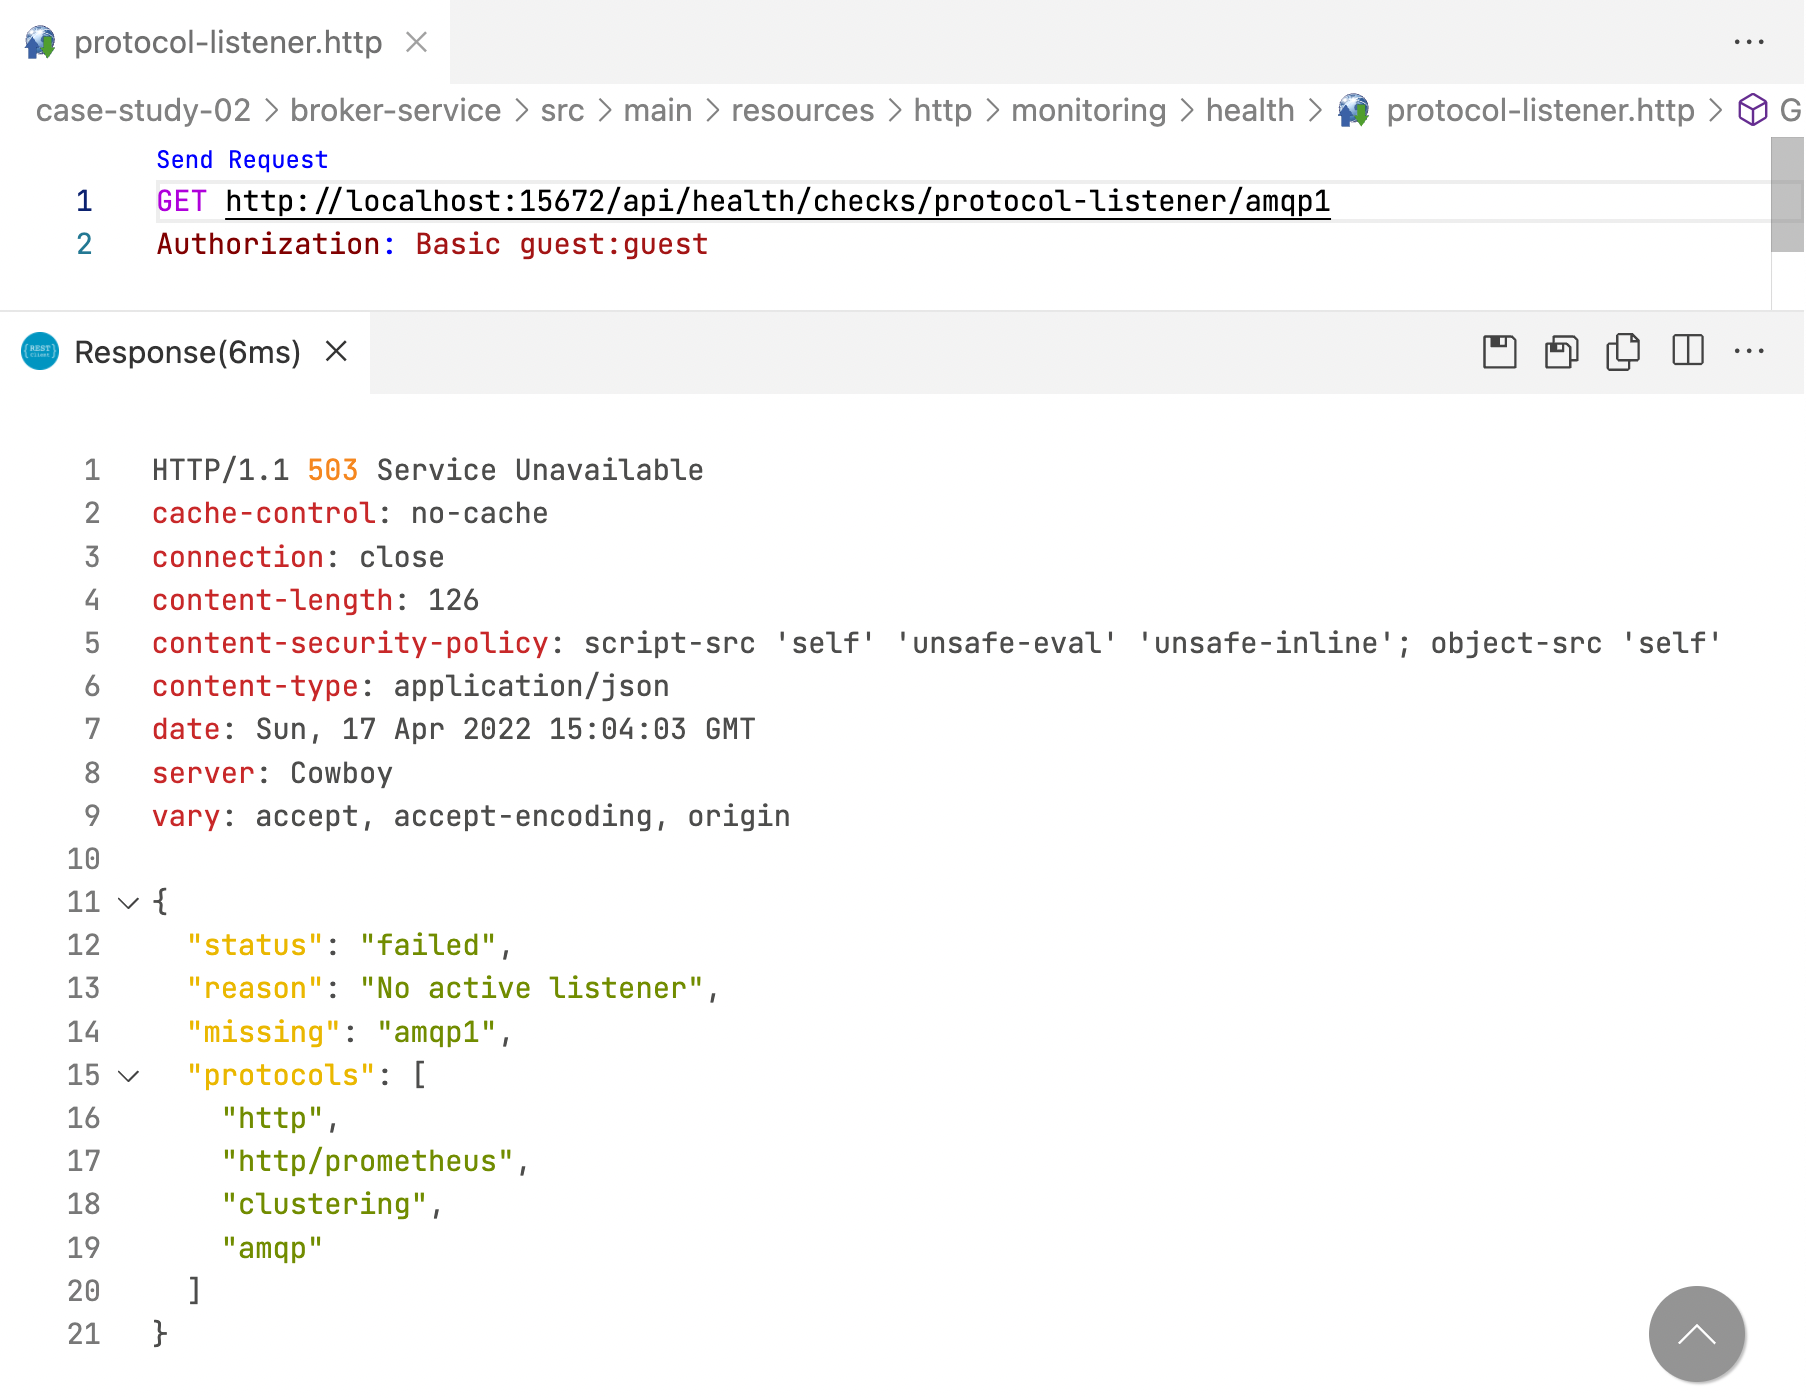
\includegraphics[width=1.0\linewidth]{./assets/images/case-studies/cs02-hc5.png}
	\caption{RabbitMQ health check - protocol listener}
	\label{fig:cs02-hc5}
\end{figure}

%%%%%%%%

\begin{figure}[H]
	\centering
	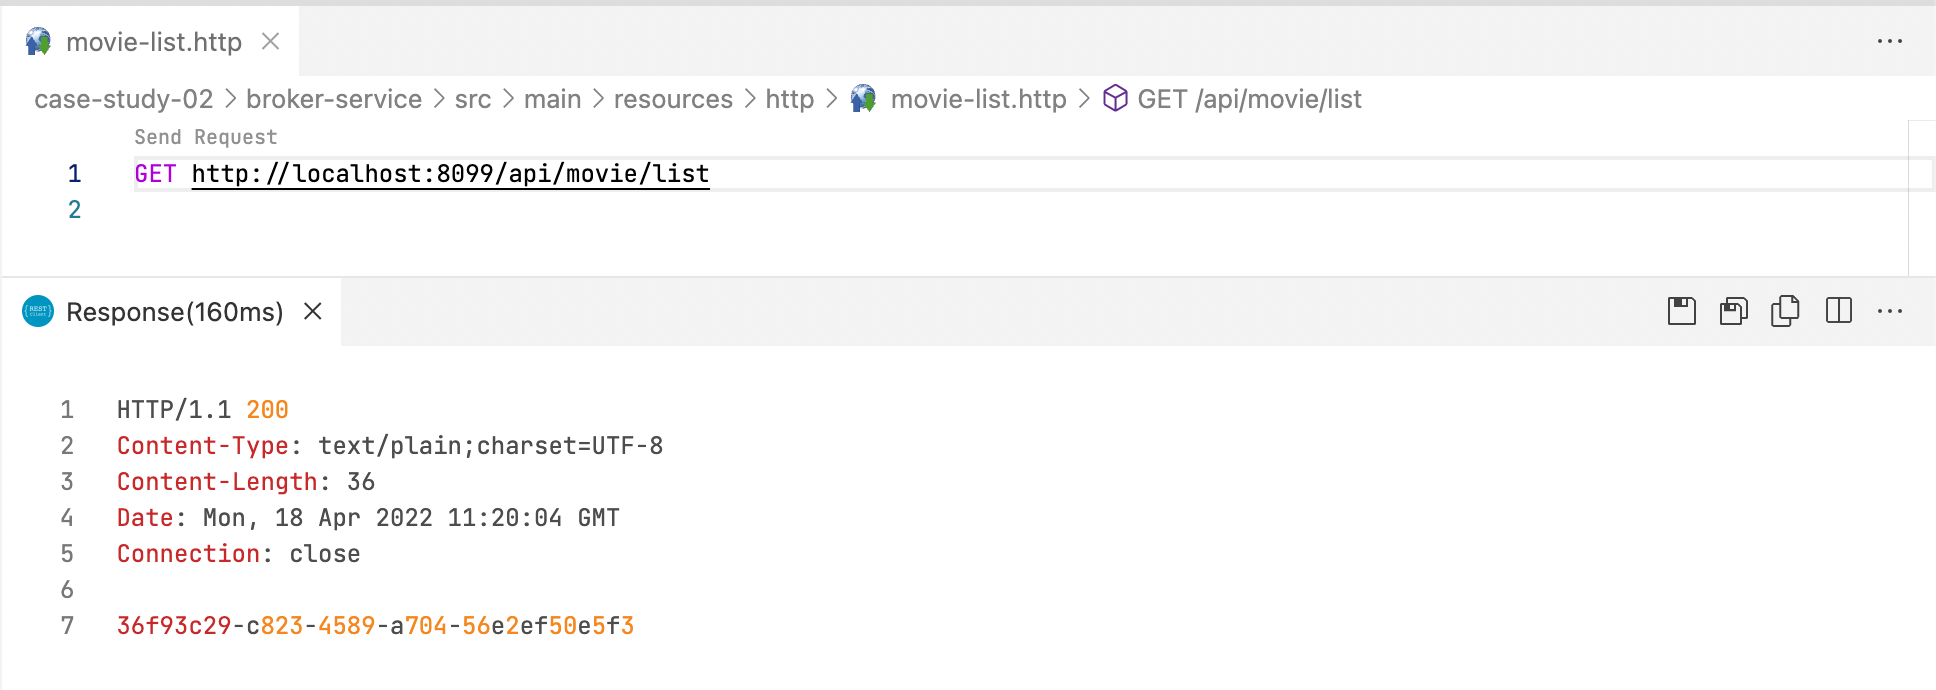
\includegraphics[width=1.0\linewidth]{./assets/images/case-studies/cs02-manual-1.png}
	\caption{Case Study 2 - manual API testing (send request to list all movies from various cinemas)}
	\label{fig:cs02-manual-1}
\end{figure}

\begin{figure}[H]
	\centering
	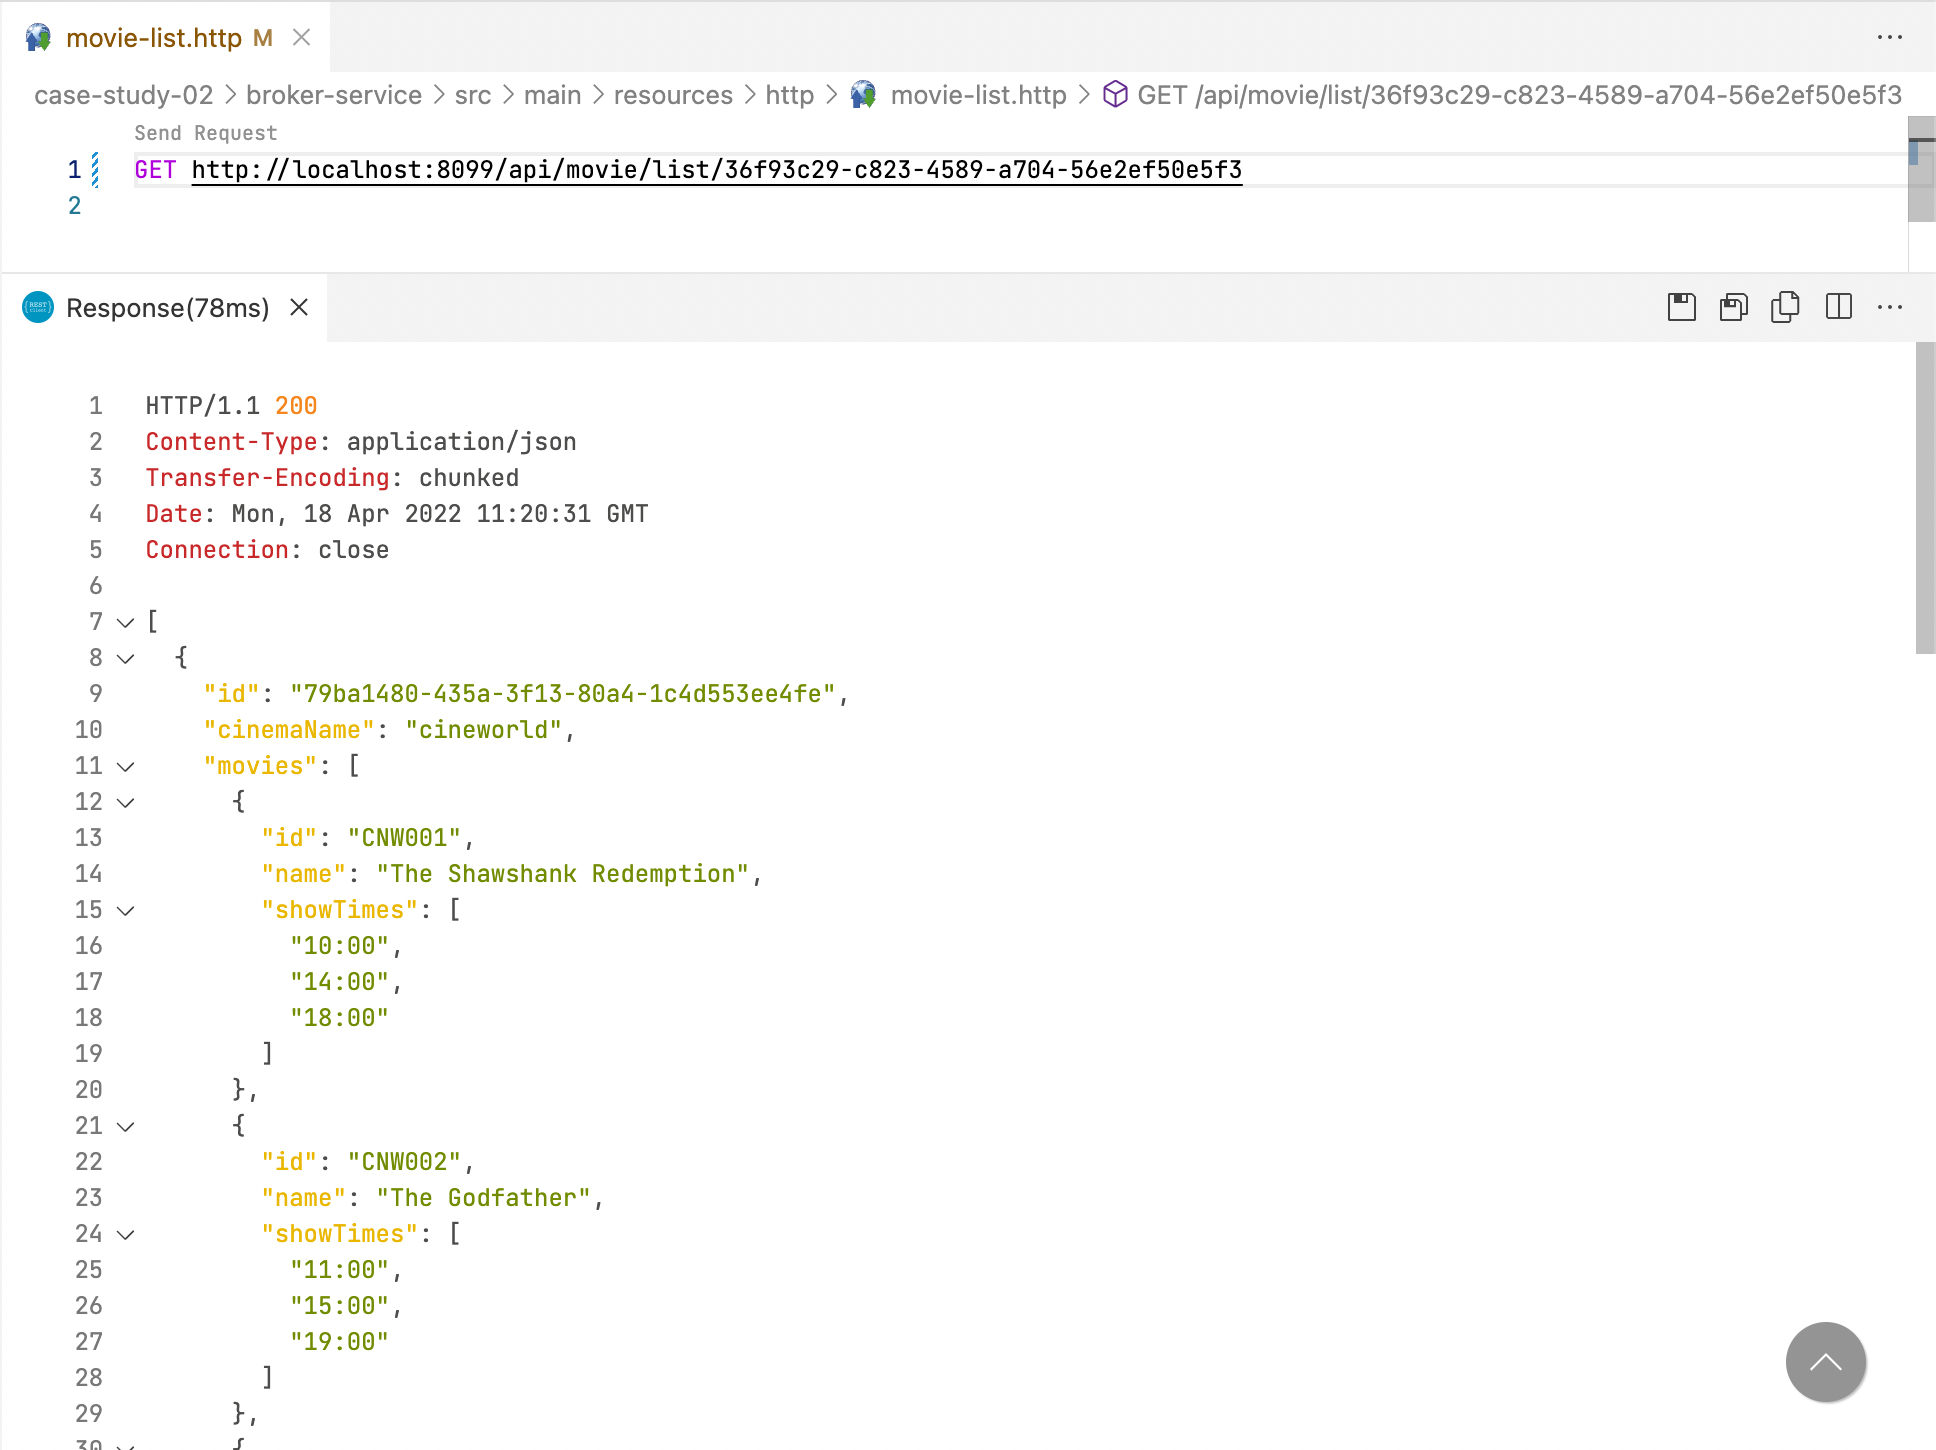
\includegraphics[width=1.0\linewidth]{./assets/images/case-studies/cs02-manual-2.png}
	\caption{Case Study 2 - manual API testing (receive response listing all movies)}
    \label{fig:cs02-manual-2}
\end{figure}

\begin{figure}[H]
	\centering
	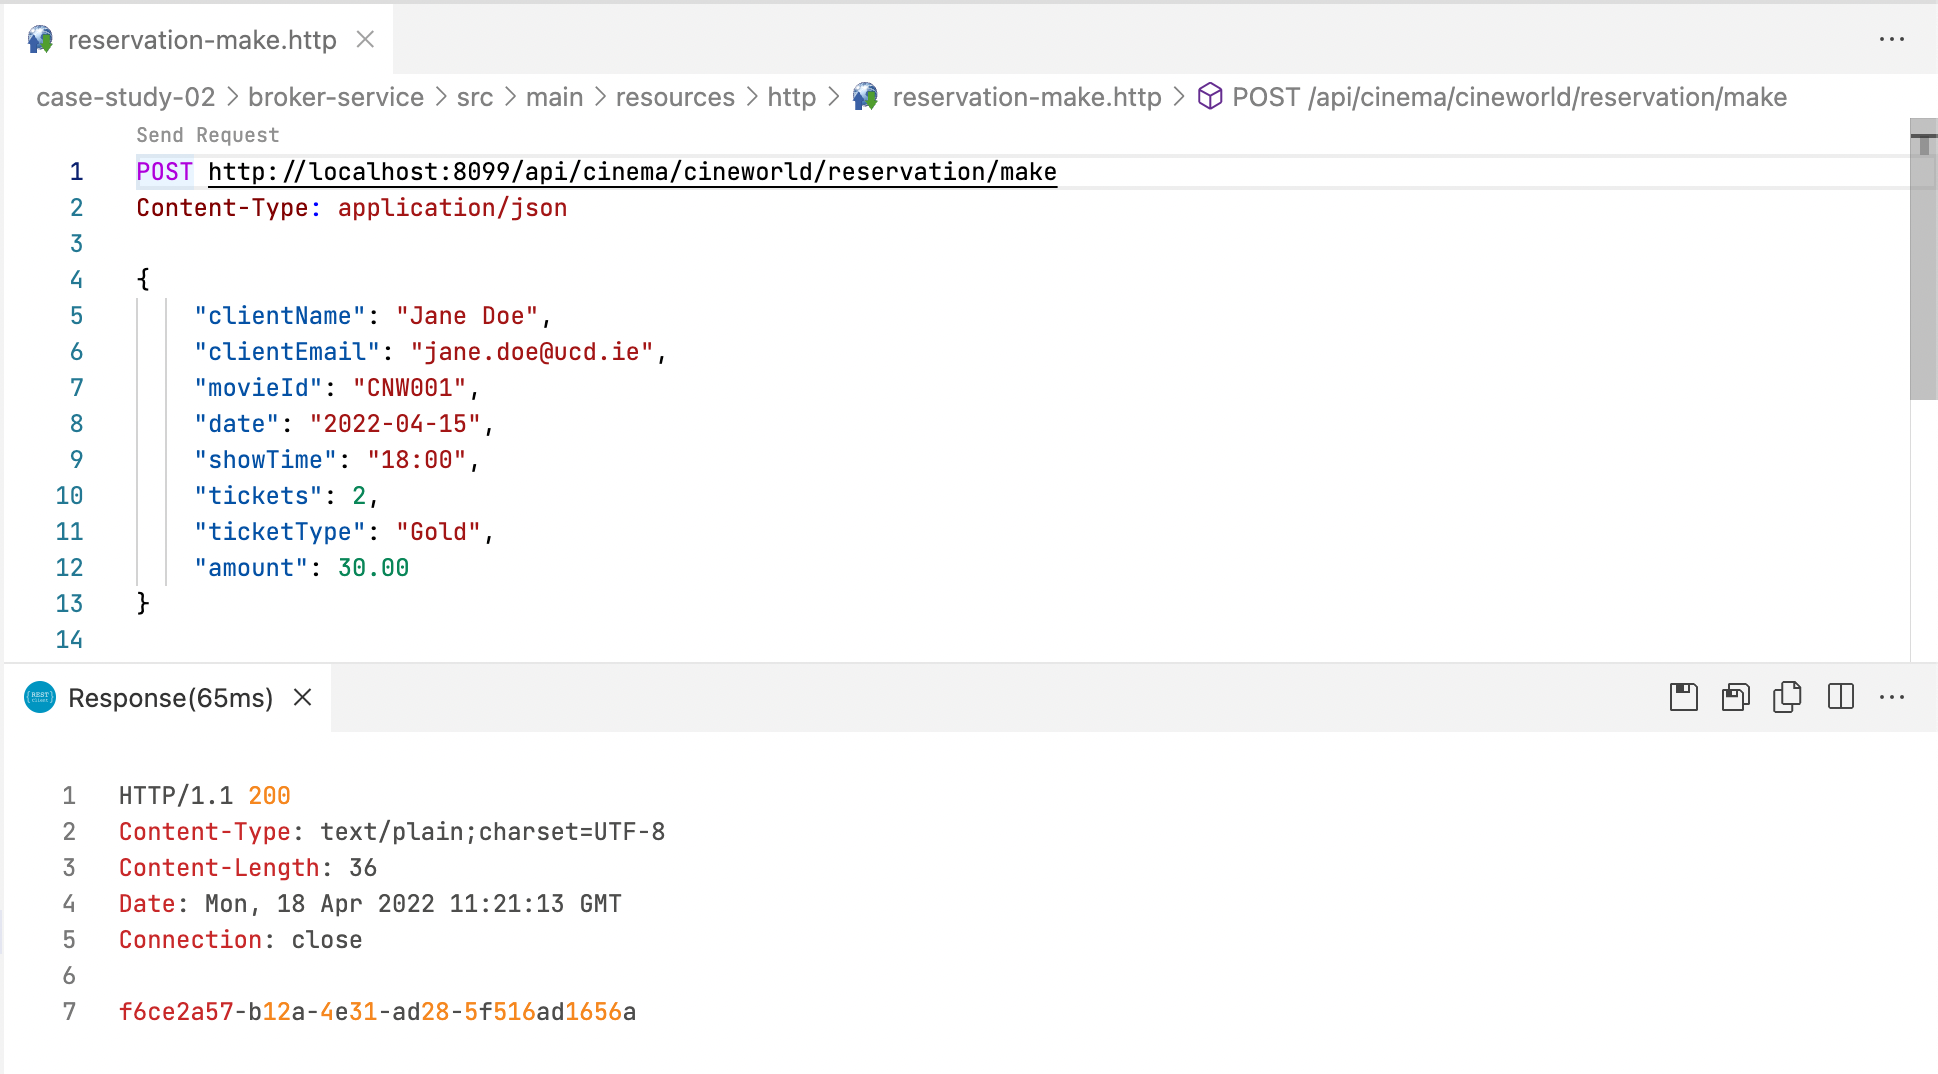
\includegraphics[width=1.0\linewidth]{./assets/images/case-studies/cs02-manual-3.png}
	\caption{Case Study 2 - manual API testing (send request to make a reservation at Cineworld cinema)}
	\label{fig:cs02-manual-3}
\end{figure}

\begin{figure}[H]
	\centering
	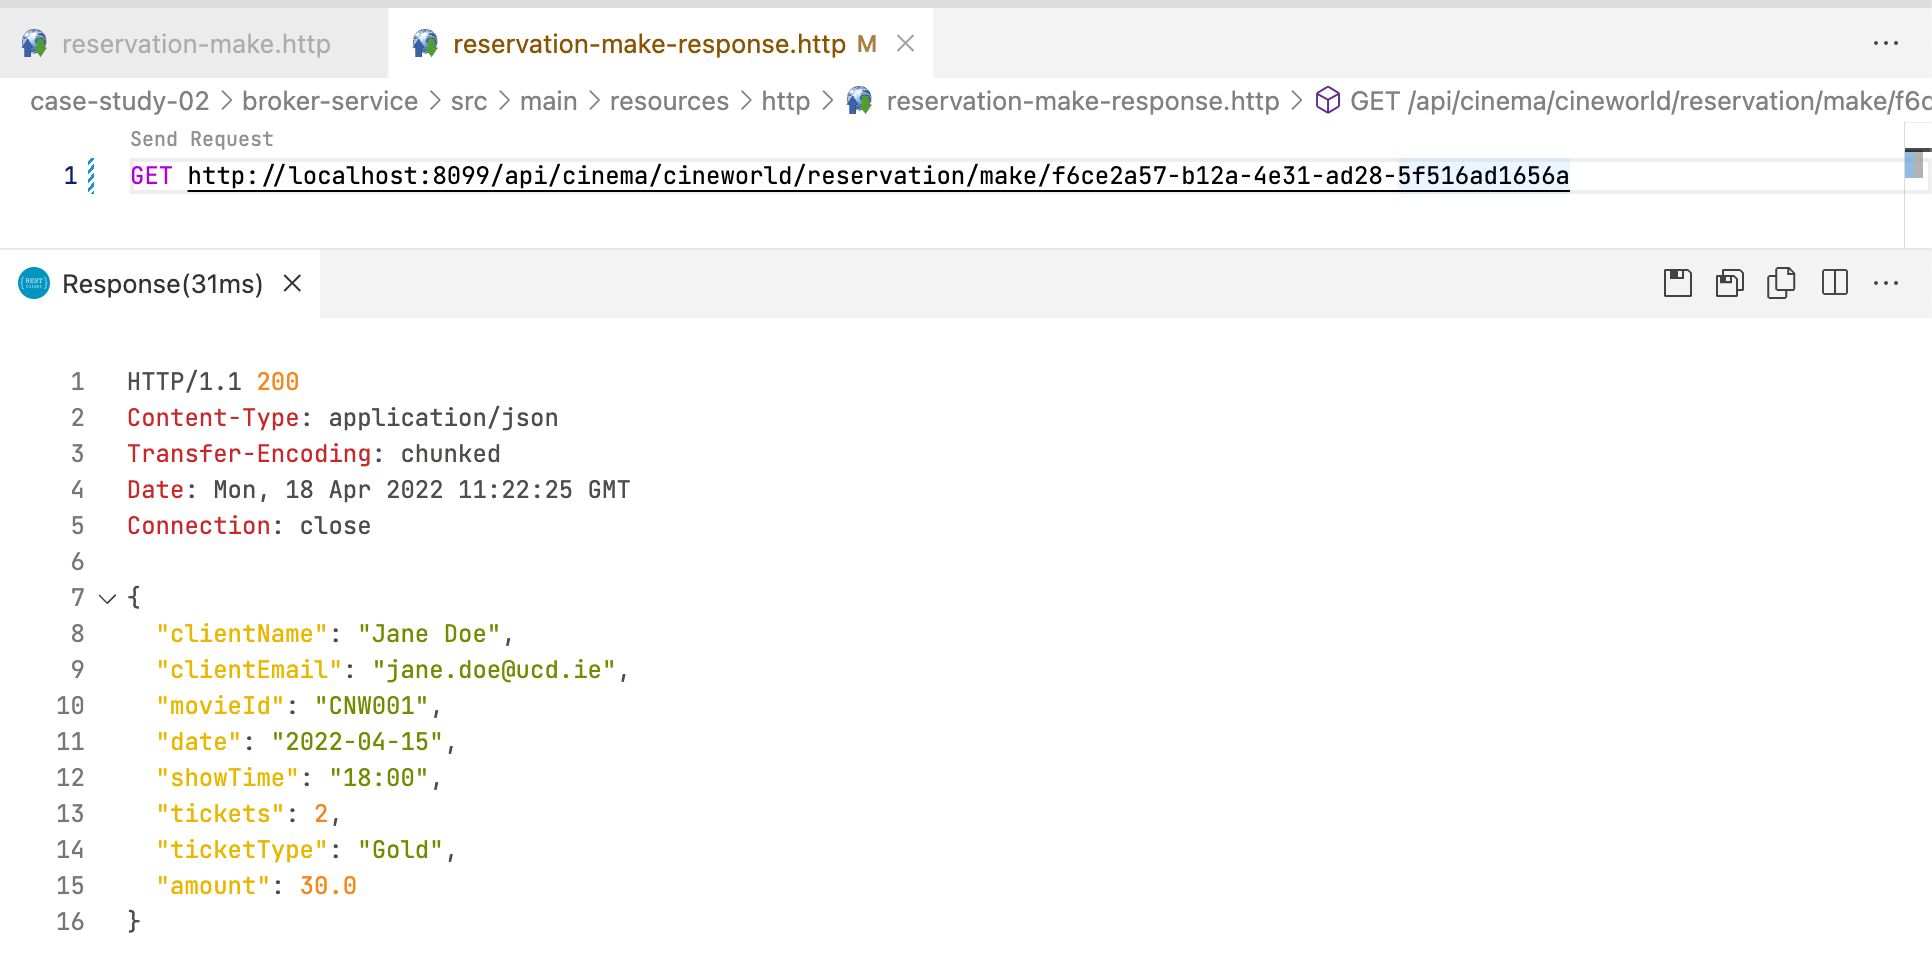
\includegraphics[width=1.0\linewidth]{./assets/images/case-studies/cs02-manual-4.png}
	\caption{Case Study 2 - manual API testing (receive response from Cineworld showing reservation)}
	\label{fig:cs02-manual-4}
\end{figure}

\begin{figure}[H]
	\centering
	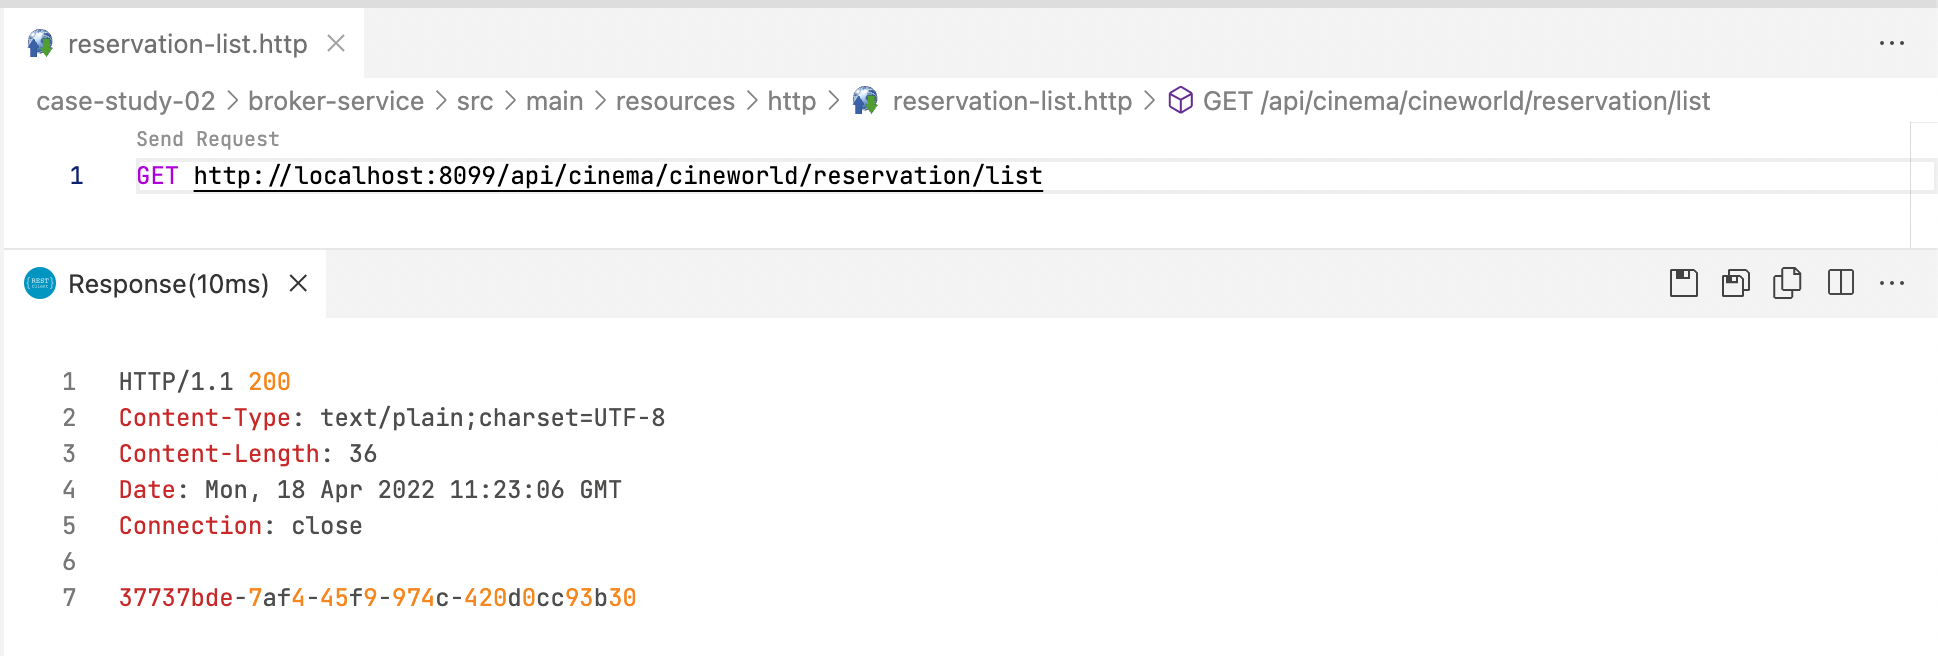
\includegraphics[width=1.0\linewidth]{./assets/images/case-studies/cs02-manual-5.png}
	\caption{Case Study 2 - manual API testing (send request to list all reservations at Cineworld)}
	\label{fig:cs02-manual-5}
\end{figure}

\begin{figure}[H]
	\centering
	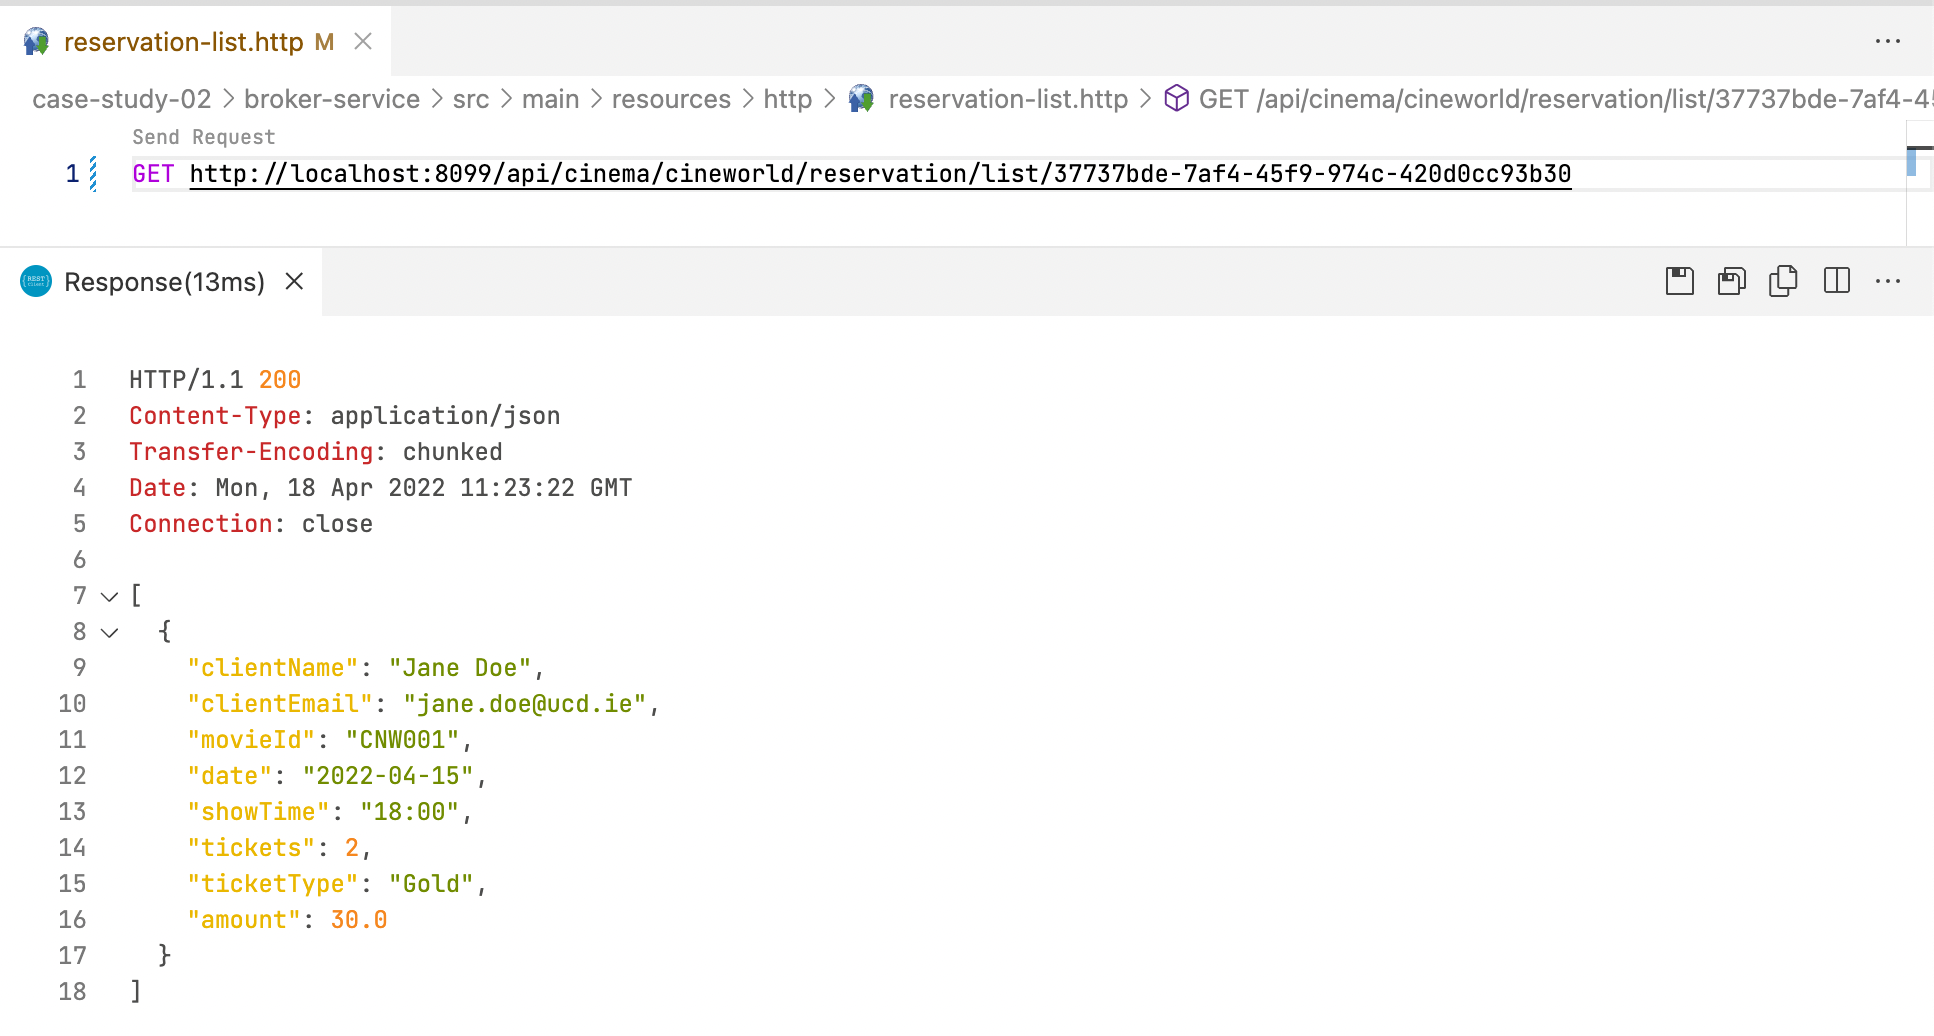
\includegraphics[width=1.0\linewidth]{./assets/images/case-studies/cs02-manual-6.png}
	\caption{Case Study 2 - manual API testing (receive response showing all of Cineworld's reservations)}
	\label{fig:cs02-manual-6}
\end{figure}

%%%%%%%%

\chapter{Project Work Plan}

\begin{figure}[h]
	\centering
	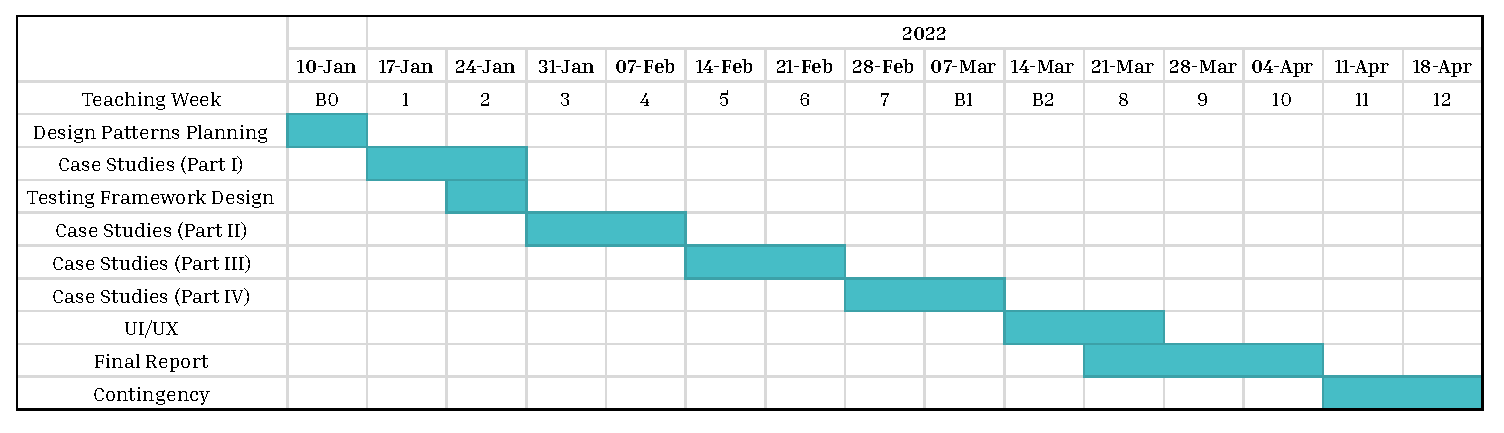
\includegraphics[width=1.0\linewidth]{./assets/images/work-plan-gantt.pdf}
	\caption{Gantt chart for project timeline}
	\label{fig:work-plan-gantt}
\end{figure}

\begin{itemize}
	\item \textbf{Design Patterns Planning (1 week)}: The initial planning here is of particular significance and will decide the direction and pace of the project's implementation phase. Various microservice design patterns will be considered to select a few important patterns which can be easily demonstrated using simulations, and then performance tested.

	\item \textbf{Testing Framework Design (1 week)}: Designing a simple testing framework (e.g. load testing plans) during the first case study will facilitate the adoption of similar strategies for subsequent case studies. 

	\item \textbf{Case Studies (Parts I, II, III, IV) (8 weeks)}: These case studies will form the bulk of the project, and will be split into four parts for convenience, each comprising a set of related design patterns (each group of case studies will possibly address 2-3 patterns). The majority of effort required here will be concerned with the back-end development of dummy microservice-based systems using containers (Docker). Evaluation, both qualitative and quantitative, is well integrated with the implementation phase of the project, since performance analysis/testing will be carried out in tandem with the case study experiments. Different configurations used during performance testing will facilitate the discussion around suitability and aptness of a number of microservice design patterns.

	\item \textbf{UI/UX (2 weeks)}: A simple web user interface will be designed to visualise the results of performance testing conducted for microservices during the different case studies, and also provide a cost-benefit analysis of the design patterns under investigation.

	\item \textbf{Final Report (3 weeks)}: Although the core parts of the report should be written as progress is made with tasks, a dedicated period is set aside for refinement and completion.

	\item \textbf{Contingency (2 weeks)}: Time set aside to be used only in the event of unforeseen issues or challenges.
\end{itemize}



